\documentclass{simple}

\title[Plapuma și coruperea]{Plapuma și coruperea}
\institute{Excursie PRECIS 708 și prietenii}
\author[Răzvan Deaconescu]{Răzvan Deaconescu \\
razvan.deaconescu@upb.ro}
\date{25 februarie 2022}

\begin{document}

\frame{\titlepage}

\begin{frame}{}
  \begin{figure}
    \centering
    \pause
    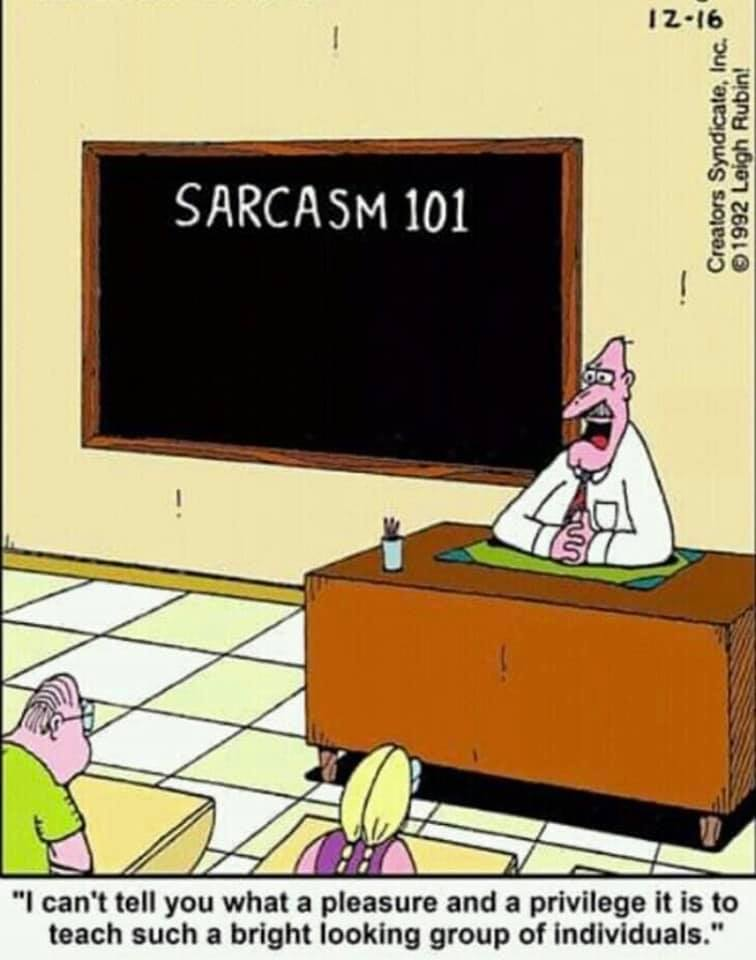
\includegraphics[width=0.6\textwidth]{img/sarcasm101.jpg}
  \end{figure}
\end{frame}

\begin{frame}{}
  \centering
  \Large{Mărturisire}
\end{frame}

\begin{frame}{}
  \pause
  \centering
  \LARGE{\textit{War... War never changes.}} \\
  \vspace{3mm}
  \hfill \normalsize{\textit{Fallout (game series)}} \\
  \vspace{1cm}
  \pause
  \centering
  \LARGE{\textit{Make no mistake, war is coming. With all its glory... and all its horror.}} \\
  \vspace{3mm}
  \hfill \normalsize{\textit{Arcturus Mengsk (Starcraft 2)}} \\
\end{frame}

\begin{frame}{Părțile bune ale unui război}
  \pause
  \centering
  \LARGE{Distruge utopiile pacifiste. Trezește lumea la realitate.} \\
  \vspace{1cm}
  \pause
  \centering
  \LARGE{Are rol de turnesol. Arată ce crede cu adevărat cineva, câți bani face, câtă coloană are, care sunt adevăratele intenții. True colors.}
\end{frame}

\begin{frame}{True Colors}
  \begin{figure}
    \centering
    \pause
    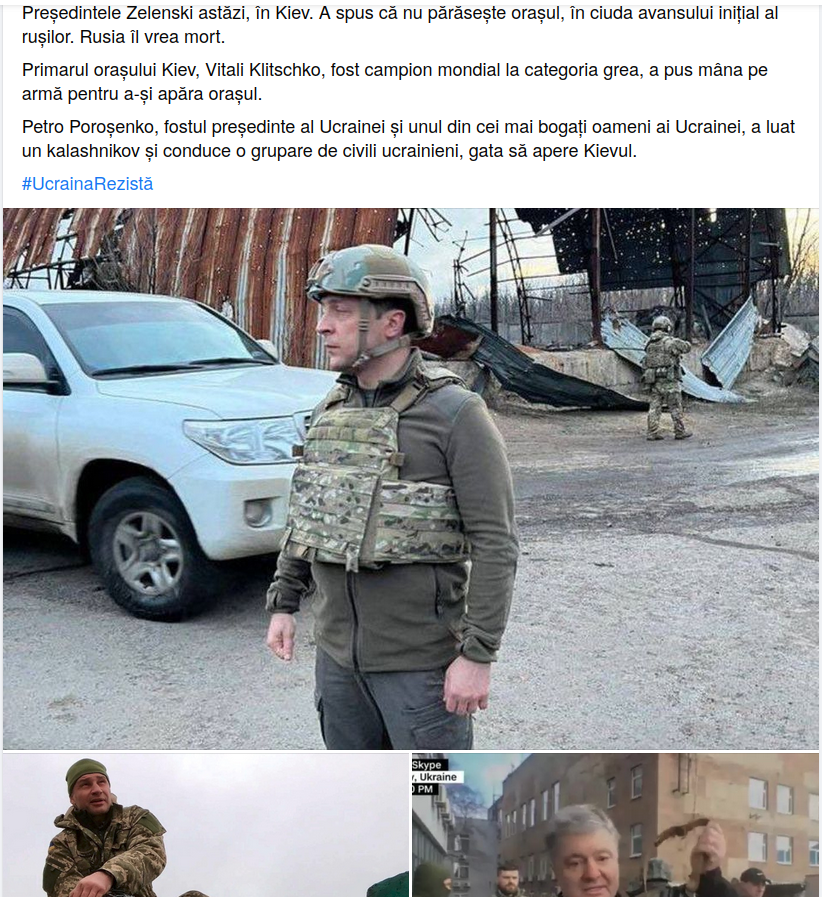
\includegraphics[width=0.7\textwidth]{img/ukrainian-leaders.png}
  \end{figure}
\end{frame}

\begin{frame}{Subiectele acestei prezentări}
  \begin{enumerate}
    \item guvernul / statul
    \item mediul economic / firmele
    \item oamenii și institutele de cultură
    \item mediul academic-intelectual
    \item divertisment / sport
    \item presă
    \item ingineri / mediu tehnologic
    \item biserică / organizațiile de cult religios
  \end{enumerate}
\end{frame}

\begin{frame}{But first ...}
  \begin{itemize}
    \pause \item Ar trebui ca o companie să decidă să nu mai facă afaceri cu companii rusești?
    \pause \item Ar trebui ca board-ul concursului ICPC (ACM) să decidă să fie excluse echipe rusești?
  \end{itemize}
\end{frame}

\begin{frame}{Checks and Balances}
  \begin{figure}
    \centering
    \pause
    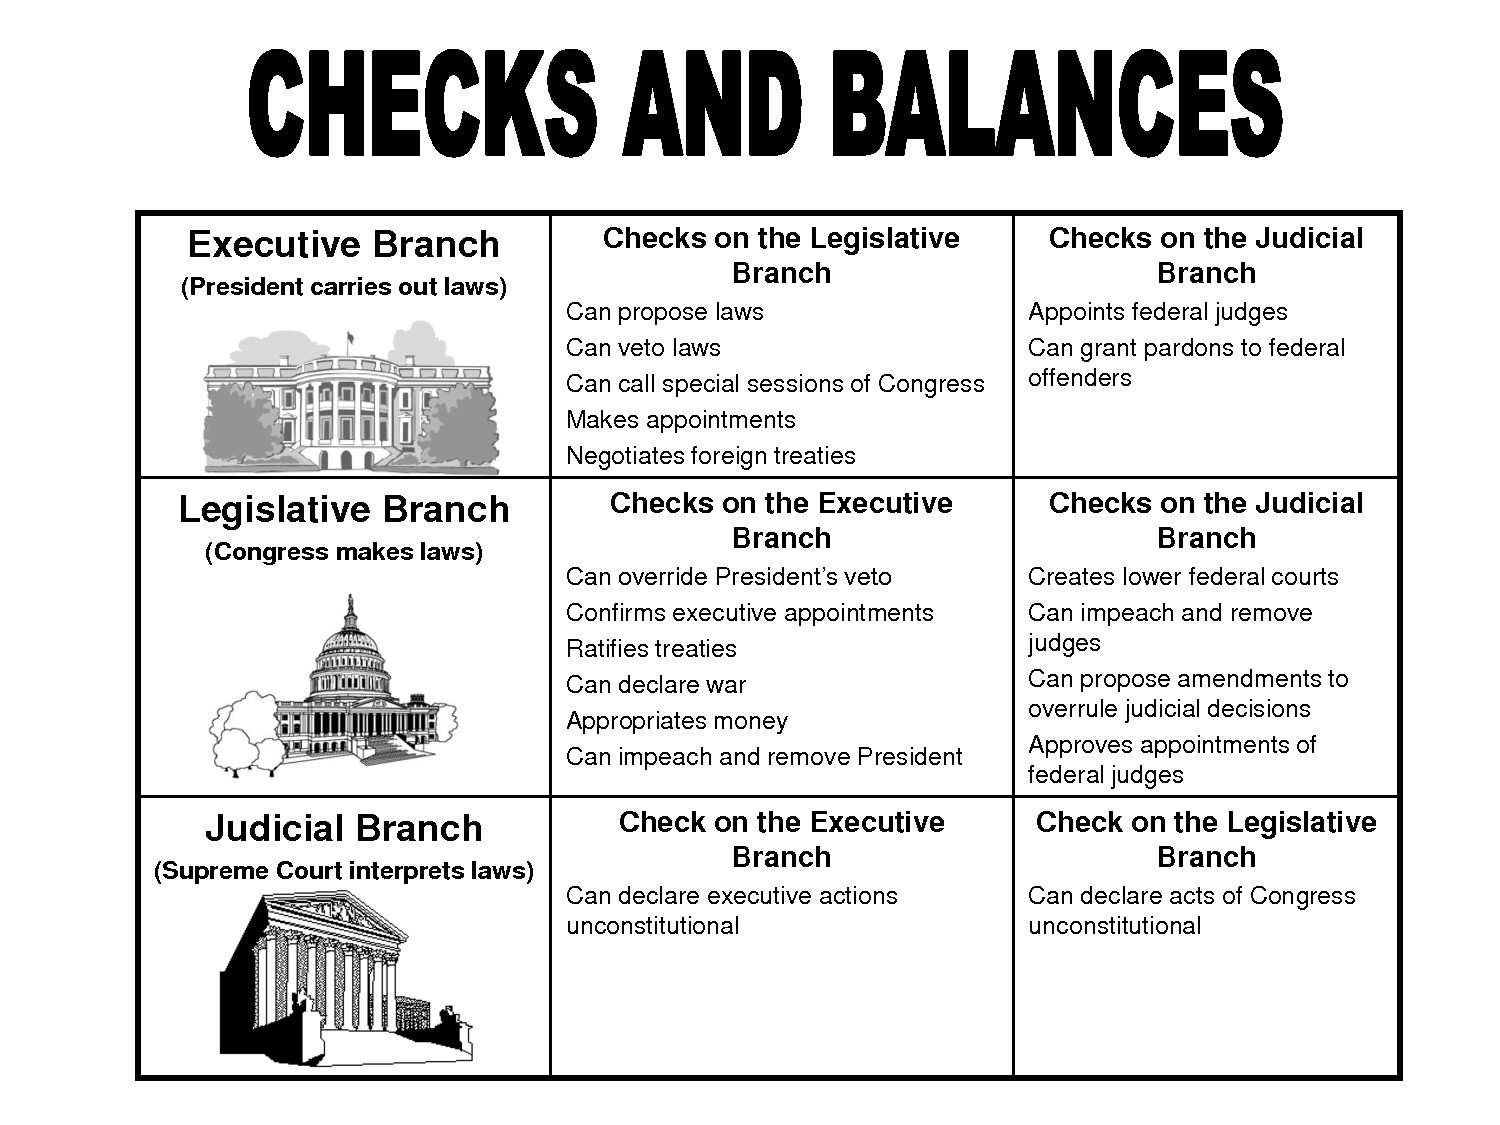
\includegraphics[width=0.9\textwidth]{img/checks-and-balances.jpg}
  \end{figure}
\end{frame}

\begin{frame}{Roluri / obiective și mijloace (1)}
  guvernul / statul
  \begin{itemize}
    \pause \item rol: pace / coeziune socială
    \pause \item mijloace: legi, taxe, servicii sociale, mediere / justiție, armată
  \end{itemize}
\end{frame}

\begin{frame}{Roluri / obiective și mijloace (2)}
  mediul economic / firmele
  \begin{itemize}
    \pause \item rol: dezvoltare economică
    \pause \item mijloace: realizarea de profit, dezvoltare tehnologică, tranzacții cu alte firme, proprietate privată (inclusiv intelectuală)
  \end{itemize}
\end{frame}

\begin{frame}{Roluri / obiective și mijloace (3)}
  oamenii și institutele de cultură
  \begin{itemize}
    \pause \item rol: dezvoltarea unei culturi (naționale, regionale)
    \pause \item mijloace: evenimente de cultură, opere de artă
  \end{itemize}
\end{frame}

\begin{frame}{Roluri / obiective și mijloace (4)}
  mediul academic-intelectual
  \begin{itemize}
    \pause \item rol: dezvoltare intelectuală, educație, căutarea ,,adevărului''
    \pause \item mijloace: cercetare științifică, critică, dezbatere, detașare
  \end{itemize}
\end{frame}

\begin{frame}{Roluri / obiective și mijloace (5)}
  divertisment / sport
  \begin{itemize}
    \pause \item rol: stare de bine, relaxare
    \pause \item mijloace: evenimente sportive și de divertisment, performanță sportivă / artistică
  \end{itemize}
\end{frame}

\begin{frame}{Roluri / obiective și mijloace (6)}
  presă
  \begin{itemize}
    \pause \item rol: informare, prezentarea ,,adevărului''
    \pause \item mijloace: investigații, articole de știri, interviuri, căutarea acului în nodul cu fân
  \end{itemize}
\end{frame}

\begin{frame}{Roluri / obiective și mijloace (7)}
  ingineri / mediu tehnologic
  \begin{itemize}
    \pause \item rol: dezvoltare tehnologică
    \pause \item mijloace: cercetare, invenții, teste / încercări, optimizări
  \end{itemize}
\end{frame}

\begin{frame}{Roluri / obiective și mijloace (8)}
  biserica / organizații de cult
  \begin{itemize}
    \pause \item rol: coeziune socială, sprijin spiritual
    \pause \item mijloace: prozelitism, lăcașe de cult, dogme, presiune socială
  \end{itemize}
\end{frame}

\begin{frame}{Dezbatere}
  \pause
  \centering
  \LARGE{Q: Trăim într-o lume dreaptă / justă / corectă?}\\
  \vspace{1cm}
  \pause
  \LARGE{A: Cu ce comparăm?}
\end{frame}

\begin{frame}{The Visual History of Decreasing War and Violence}
  \centering
  \url{https://slides.ourworldindata.org/war-and-violence/}
\end{frame}

\begin{frame}{}
  \pause
  \centering
  \LARGE{Q: Ce procentaj dintre profesori are feedback peste 4 (din 5)? Dar cursuri?}\\
  \vspace{1cm}
  \pause
  \LARGE{A: Peste 60\%. Peste 40\%.}
\end{frame}

\begin{frame}{De ce perspectiva negativistă / justițiară?}
  \begin{itemize}
    \pause \item emoțiile ,,negative'' se ,,vând'' bine
    \pause \item emoțiile ,,negative'' se întipăresc
    \pause \item Internetul: afli multe (negative)
    \pause \item mult timp la dispoziție; trecerea de la subzistență la activism
  \end{itemize}
\end{frame}

\begin{frame}{Și ... ce?}
  \begin{itemize}
    \pause \item presiune / activism pe ,,subiecte'' să aibă metode / mijloace / metrici de ,,dreptate'' / ,,fairness''
    \pause \item aceste mijloace sunt dincolo de \textbf{plapuma} subiectului
    \pause \item ,,nu-l ține plapuma''; efectul este \textbf{coruperea} rolului
  \end{itemize}
\end{frame}

\begin{frame}{Billions (s06e04)}
  \centering
  \LARGE{video pe HBO GO}
\end{frame}

\begin{frame}{Decolonizing Chemistry}
  \begin{figure}
    \centering
    \pause
    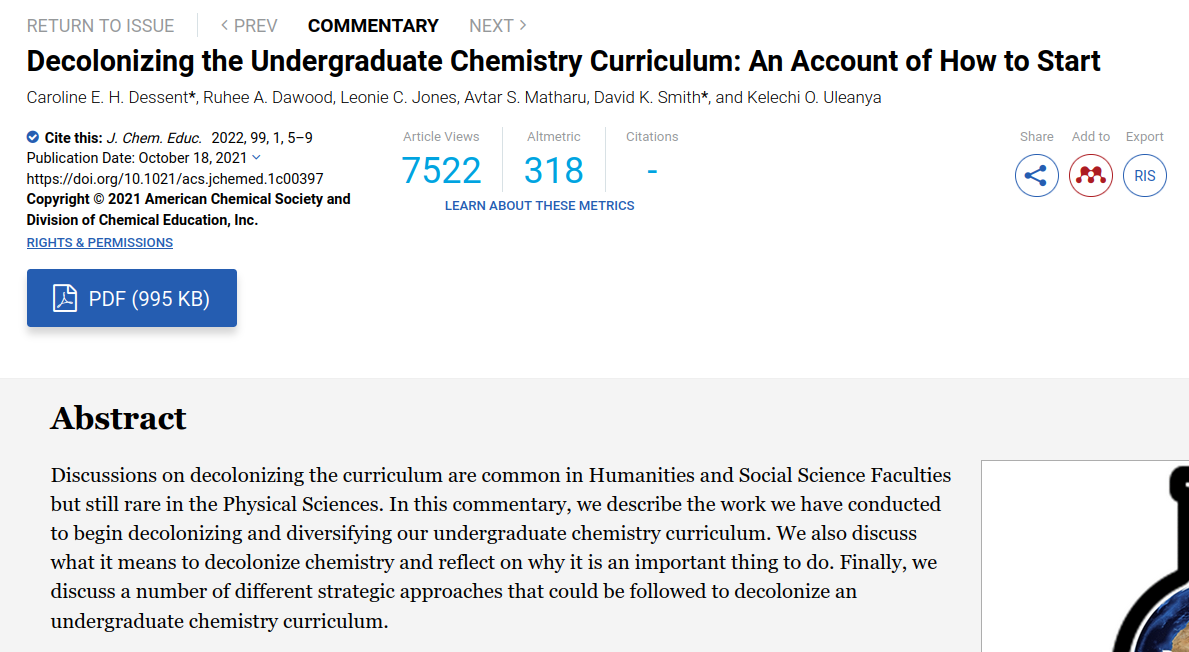
\includegraphics[width=0.8\textwidth]{img/decolonizing-chemistry.png}
  \end{figure}
  \begin{center}
    \tiny
    \url{http://www.imediaethics.org/wp-content/uploads/2015/12/lovetrumpshate.jpg}
  \end{center}
\end{frame}

\begin{frame}{Libraries}
  {\tiny
  \url{https://quillette.com/2022/02/06/watching-my-beloved-once-eclectic-library-become-just-another-bastion-of-orthodoxy/}
  }
  \begin{figure}
    \centering
    \pause
    
\includegraphics[width=0.5\textwidth]{img/library-offend.jpg}
  \end{figure}
\end{frame}

\begin{frame}{Bashing Neil deGrasse Tyson}
  \begin{figure}
    \centering
    \pause
    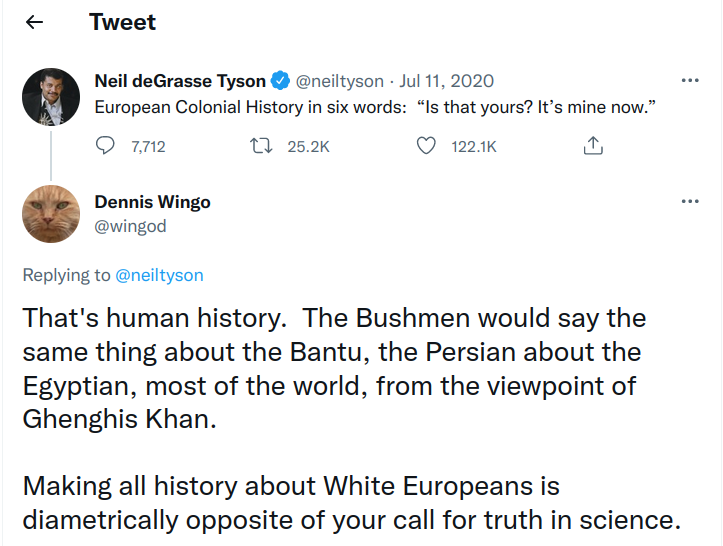
\includegraphics[width=0.8\textwidth]{img/neil-degrasse-tyson-wingod.png}
  \end{figure}
  \begin{center}
    \tiny
    \url{https://twitter.com/wingod/status/1281812815028686851}
  \end{center}
\end{frame}

\begin{frame}{Plapuma și coruperea}
  \begin{itemize}
    \pause \item nu există perfecțiune, există iterație
    \pause \item trăim în cele mai bune vremuri ale omenirii
    \pause \item drumul spre iad e pavat cu bune intenții
    \pause \item dacă un subiect își depășește plapuma, riscă să-și corupă rolul în societate
    \pause \item sistemul de check and balances are efect (dar durează)
    \pause \item răbdare, semințe și tutun
  \end{itemize}
\end{frame}

\begin{frame}{Concluzii}
  \centering
  \pause
  \LARGE{Fiecare și le trage singur.}
\end{frame}

\end{document}
